\documentclass[border=8pt]{standalone}
\usepackage[T1]{fontenc}\usepackage{helvet}\renewcommand{\familydefault}{\sfdefault}
\usepackage{tikz}\usetikzlibrary{arrows.meta, positioning, calc, backgrounds}
\definecolor{ink}{HTML}{1a1916}
\definecolor{inktwo}{HTML}{3a3a35}
\definecolor{inkthree}{HTML}{6a6862}
\definecolor{rule}{HTML}{b8b09a}
\definecolor{amber}{HTML}{a8730a}
\definecolor{red}{HTML}{c8261a}
\definecolor{paper}{HTML}{f0eee5}
\definecolor{slab}{HTML}{d8d4c6}
\tikzset{
  >={Stealth[length=2.2mm]},
  wire/.style={line width=0.8pt, ink},
  modwire/.style={line width=0.6pt, dashed, ink},
  tastewire/.style={line width=0.6pt, dashed, amber},
  gatewire/.style={line width=0.6pt, dotted, ink},
  block/.style={rectangle, draw=ink, line width=0.9pt, fill=slab, minimum width=3.0cm, minimum height=1.9cm, inner sep=0pt},
  perf/.style={rectangle, draw=ink, line width=0.7pt, minimum width=3.0cm, minimum height=0.7cm, inner sep=2pt, font=\footnotesize, text=ink},
  title/.style={font=\scriptsize\bfseries, text=ink, anchor=north, inner sep=2pt},
  jack/.style={circle, draw=ink, fill=paper, line width=0.5pt, minimum size=3.2pt, inner sep=0pt},
  plabel/.style={font=\tiny, text=inktwo, anchor=west, inner sep=1pt},
  olabel/.style={font=\tiny, text=inktwo, anchor=east, inner sep=1pt},
  settings/.style={font=\scriptsize, text=ink, align=left, anchor=north west, inner sep=1pt, text width=2.9cm},
}
\begin{document}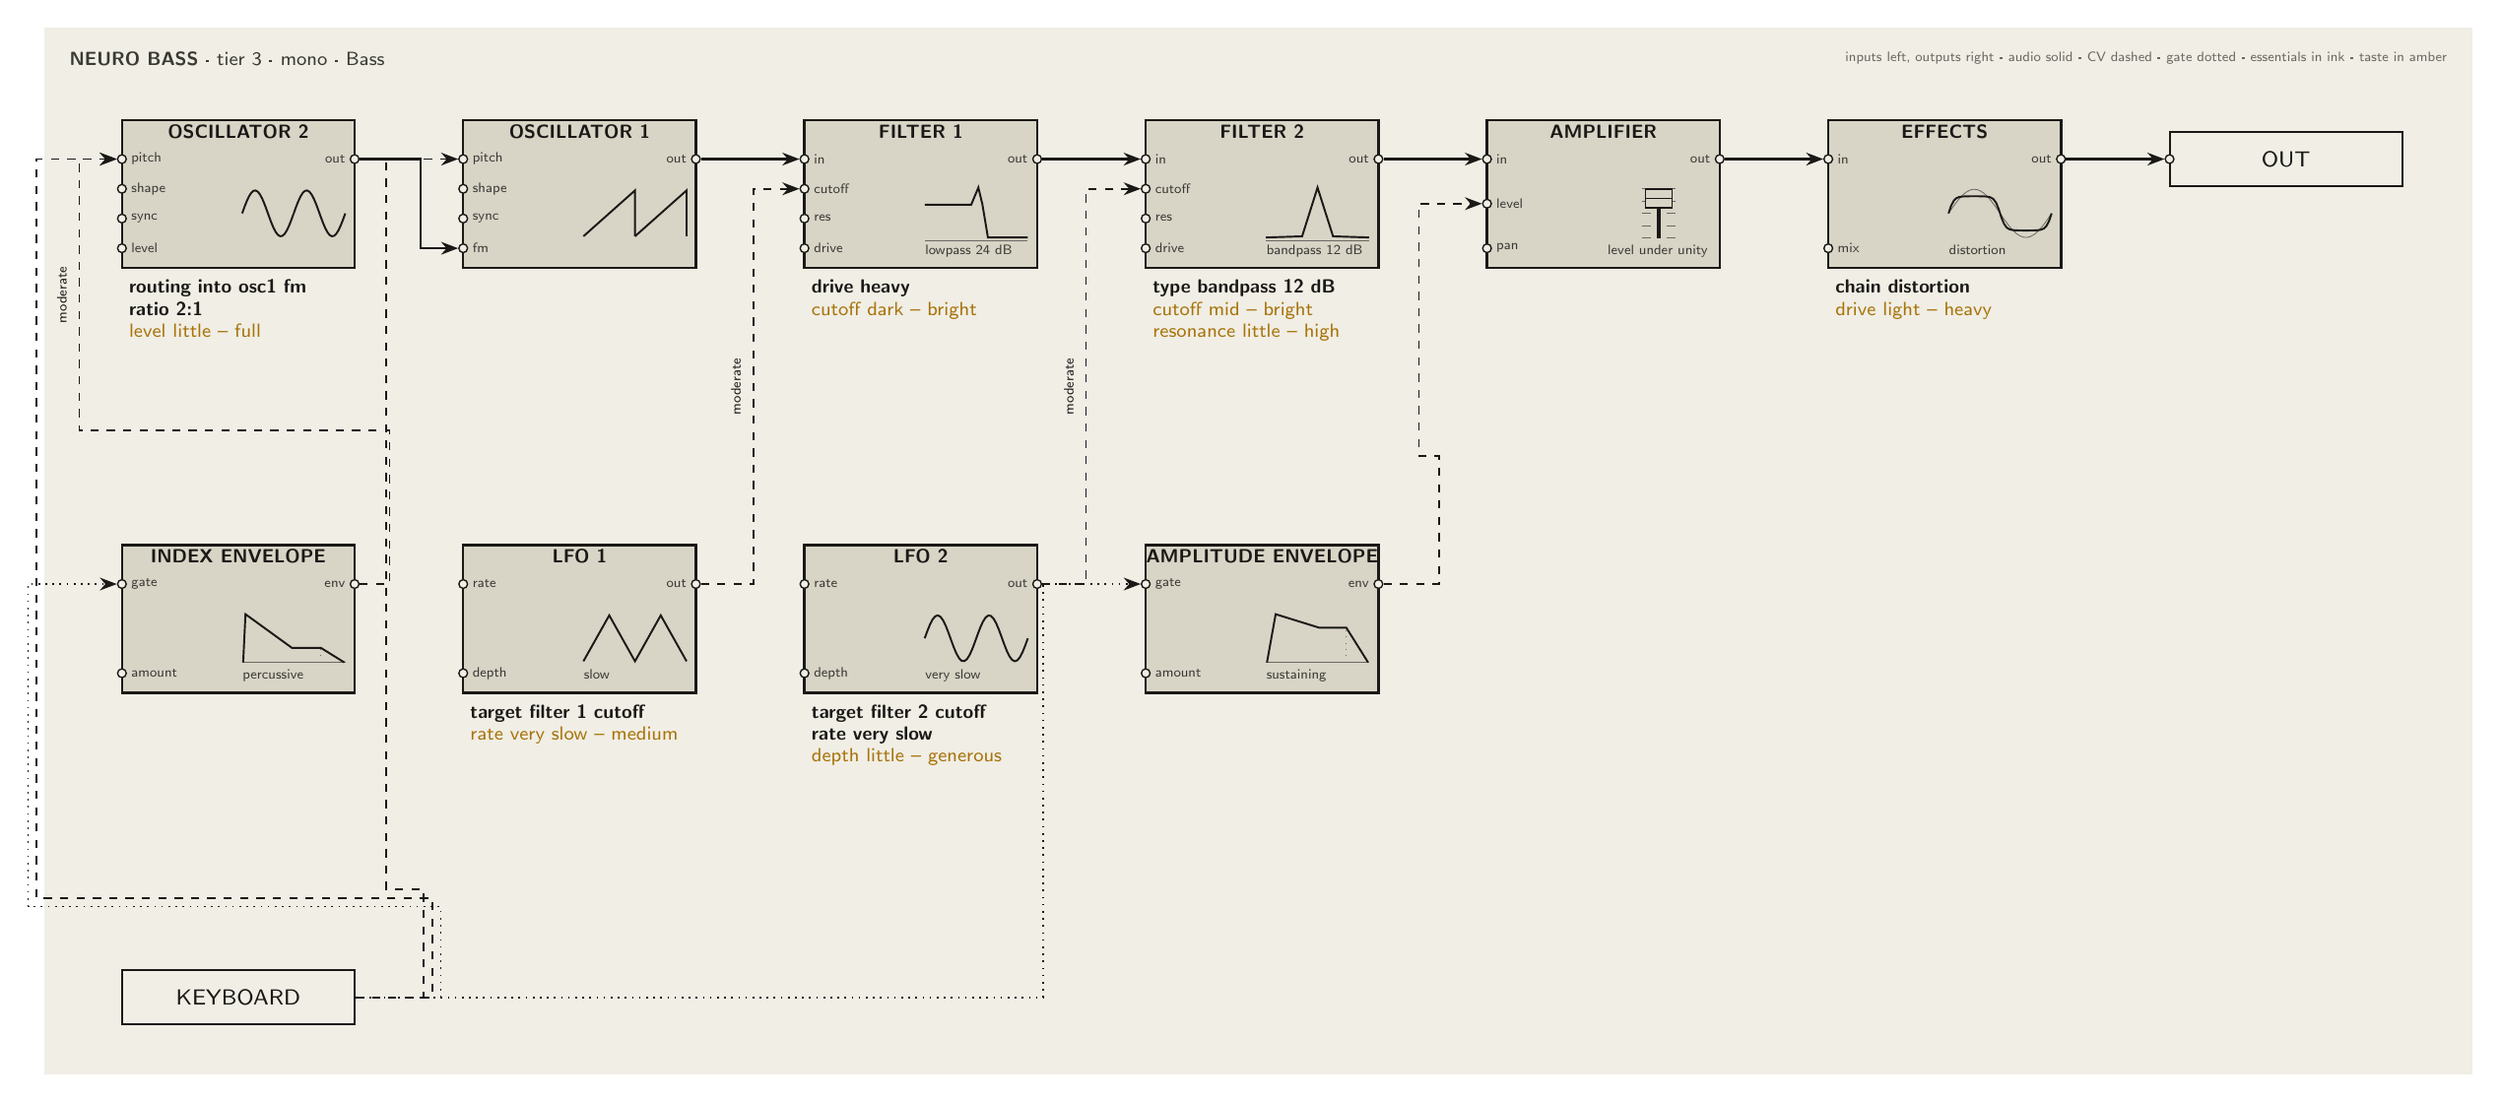
\begin{tikzpicture}
\begin{scope}[on background layer]\fill[paper] (-2.5,-11.36) rectangle (28.8,2.15);\end{scope}
\node[block, minimum height=1.9cm] (osc1) at (4.4,0.0) {};
\node[title] at (osc1.north) {OSCILLATOR 1};
\node[jack] (osc1-pitch) at (2.9000000000000004,0.44999999999999996) {};
\node[plabel] at (2.9800000000000004,0.44999999999999996) {pitch};
\node[jack] (osc1-shape) at (2.9000000000000004,0.06666666666666665) {};
\node[plabel] at (2.9800000000000004,0.06666666666666665) {shape};
\node[jack] (osc1-sync) at (2.9000000000000004,-0.31666666666666665) {};
\node[plabel] at (2.9800000000000004,-0.31666666666666665) {sync};
\node[jack] (osc1-fm) at (2.9000000000000004,-0.7) {};
\node[plabel] at (2.9800000000000004,-0.7) {fm};
\node[jack] (osc1-out) at (5.9,0.44999999999999996) {};
\node[olabel] at (5.82,0.44999999999999996) {out};
\begin{scope}
\draw[ink, line width=0.7pt] (4.450,-0.546) -- (5.115,0.046) -- (5.115,-0.546);
\draw[ink, line width=0.7pt] (5.115,-0.546) -- (5.780,0.046) -- (5.780,-0.546);
\end{scope}
\node[block, minimum height=1.9cm] (osc2) at (0.0,0.0) {};
\node[title] at (osc2.north) {OSCILLATOR 2};
\node[jack] (osc2-pitch) at (-1.5,0.44999999999999996) {};
\node[plabel] at (-1.42,0.44999999999999996) {pitch};
\node[jack] (osc2-shape) at (-1.5,0.06666666666666665) {};
\node[plabel] at (-1.42,0.06666666666666665) {shape};
\node[jack] (osc2-sync) at (-1.5,-0.31666666666666665) {};
\node[plabel] at (-1.42,-0.31666666666666665) {sync};
\node[jack] (osc2-level) at (-1.5,-0.7) {};
\node[plabel] at (-1.42,-0.7) {level};
\node[jack] (osc2-out) at (1.5,0.44999999999999996) {};
\node[olabel] at (1.42,0.44999999999999996) {out};
\begin{scope}
\draw[ink, line width=0.7pt] plot[domain=0.000:0.500, samples=24, variable=\u] ({0.050+\u*1.330},{-0.620+(0.740)*(0.5+0.4*sin(360*(\u*2))+0.0)});
\draw[ink, line width=0.7pt] plot[domain=0.500:1.000, samples=24, variable=\u] ({0.050+\u*1.330},{-0.620+(0.740)*(0.5+0.4*sin(360*(\u*2))+0.0)});
\end{scope}
\node[settings] at (-1.45,-1.0699999999999998) {\textbf{routing into osc1 fm} \\ \textbf{ratio 2:1} \\ \textcolor{amber}{level little -- full}};
\node[block, minimum height=1.9cm] (filter1) at (8.8,0.0) {};
\node[title] at (filter1.north) {FILTER 1};
\node[jack] (filter1-in) at (7.300000000000001,0.44999999999999996) {};
\node[plabel] at (7.380000000000001,0.44999999999999996) {in};
\node[jack] (filter1-cutoff) at (7.300000000000001,0.06666666666666665) {};
\node[plabel] at (7.380000000000001,0.06666666666666665) {cutoff};
\node[jack] (filter1-res) at (7.300000000000001,-0.31666666666666665) {};
\node[plabel] at (7.380000000000001,-0.31666666666666665) {res};
\node[jack] (filter1-drive) at (7.300000000000001,-0.7) {};
\node[plabel] at (7.380000000000001,-0.7) {drive};
\node[jack] (filter1-out) at (10.3,0.44999999999999996) {};
\node[olabel] at (10.22,0.44999999999999996) {out};
\begin{scope}
\draw[inkthree, line width=0.3pt] (8.850,-0.605) -- (10.180,-0.605);
\draw[ink, line width=0.7pt] (8.850,-0.139) -- (9.449,-0.139) -- (9.542,0.083) -- (9.595,-0.139) -- (9.665,-0.561) -- (10.180,-0.561);
\node[font=\tiny, text=inktwo, anchor=north west, inner sep=0pt] at (8.850,-0.650) {lowpass 24 dB};
\end{scope}
\node[settings] at (7.3500000000000005,-1.0699999999999998) {\textbf{drive heavy} \\ \textcolor{amber}{cutoff dark -- bright}};
\node[block, minimum height=1.9cm] (filter2) at (13.200000000000001,0.0) {};
\node[title] at (filter2.north) {FILTER 2};
\node[jack] (filter2-in) at (11.700000000000001,0.44999999999999996) {};
\node[plabel] at (11.780000000000001,0.44999999999999996) {in};
\node[jack] (filter2-cutoff) at (11.700000000000001,0.06666666666666665) {};
\node[plabel] at (11.780000000000001,0.06666666666666665) {cutoff};
\node[jack] (filter2-res) at (11.700000000000001,-0.31666666666666665) {};
\node[plabel] at (11.780000000000001,-0.31666666666666665) {res};
\node[jack] (filter2-drive) at (11.700000000000001,-0.7) {};
\node[plabel] at (11.780000000000001,-0.7) {drive};
\node[jack] (filter2-out) at (14.700000000000001,0.44999999999999996) {};
\node[olabel] at (14.620000000000001,0.44999999999999996) {out};
\begin{scope}
\draw[inkthree, line width=0.3pt] (13.250,-0.605) -- (14.580,-0.605);
\draw[ink, line width=0.7pt] (13.250,-0.561) -- (13.716,-0.546) -- (13.915,0.083) -- (14.115,-0.546) -- (14.580,-0.561);
\node[font=\tiny, text=inktwo, anchor=north west, inner sep=0pt] at (13.250,-0.650) {bandpass 12 dB};
\end{scope}
\node[settings] at (11.750000000000002,-1.0699999999999998) {\textbf{type bandpass 12 dB} \\ \textcolor{amber}{cutoff mid -- bright} \\ \textcolor{amber}{resonance little -- high}};
\node[block, minimum height=1.9cm] (amp) at (17.6,0.0) {};
\node[title] at (amp.north) {AMPLIFIER};
\node[jack] (amp-in) at (16.1,0.44999999999999996) {};
\node[plabel] at (16.18,0.44999999999999996) {in};
\node[jack] (amp-level) at (16.1,-0.125) {};
\node[plabel] at (16.18,-0.125) {level};
\node[jack] (amp-pan) at (16.1,-0.7) {};
\node[plabel] at (16.18,-0.7) {pan};
\node[jack] (amp-out) at (19.1,0.44999999999999996) {};
\node[olabel] at (19.020000000000003,0.44999999999999996) {out};
\begin{scope}
\draw[ink, line width=1.2pt] (18.315,-0.570) -- (18.315,0.070);
\draw[inkthree, line width=0.3pt] (18.095,-0.570) -- (18.215,-0.570) (18.415,-0.570) -- (18.535,-0.570);
\draw[inkthree, line width=0.3pt] (18.095,-0.410) -- (18.215,-0.410) (18.415,-0.410) -- (18.535,-0.410);
\draw[inkthree, line width=0.3pt] (18.095,-0.250) -- (18.215,-0.250) (18.415,-0.250) -- (18.535,-0.250);
\draw[inkthree, line width=0.3pt] (18.095,-0.090) -- (18.215,-0.090) (18.415,-0.090) -- (18.535,-0.090);
\draw[inkthree, line width=0.3pt] (18.095,0.070) -- (18.215,0.070) (18.415,0.070) -- (18.535,0.070);
\fill[slab, draw=ink, line width=0.6pt] (18.145,-0.178) rectangle (18.485,0.062);
\draw[ink, line width=0.5pt] (18.145,-0.058) -- (18.485,-0.058);
\node[font=\tiny, text=inktwo, anchor=north west, inner sep=0pt] at (17.650,-0.650) {level under unity};
\end{scope}
\node[block, minimum height=1.9cm] (fx) at (22.0,0.0) {};
\node[title] at (fx.north) {EFFECTS};
\node[jack] (fx-in) at (20.5,0.44999999999999996) {};
\node[plabel] at (20.58,0.44999999999999996) {in};
\node[jack] (fx-mix) at (20.5,-0.7) {};
\node[plabel] at (20.58,-0.7) {mix};
\node[jack] (fx-out) at (23.5,0.44999999999999996) {};
\node[olabel] at (23.42,0.44999999999999996) {out};
\begin{scope}
\draw[inkthree, line width=0.3pt] plot[domain=0.000:1.000, samples=30, variable=\u] ({22.050+\u*1.330},{-0.620+(0.740)*(0.5+0.42*sin(360*((\u-0.000)/1.000)))});
\draw[ink, line width=0.7pt] plot[domain=0.000:1.000, samples=40, variable=\u] ({22.050+\u*1.330},{-0.620+(0.740)*(0.5+0.3*tanh(3*sin(360*((\u-0.000)/1.000))))});
\node[font=\tiny, text=inktwo, anchor=north west, inner sep=0pt] at (22.050,-0.650) {distortion};
\end{scope}
\node[settings] at (20.55,-1.0699999999999998) {\textbf{chain distortion} \\ \textcolor{amber}{drive light -- heavy}};
\node[block, minimum height=1.9cm] (menv) at (0.0,-5.4799999999999995) {};
\node[title] at (menv.north) {INDEX ENVELOPE};
\node[jack] (menv-gate) at (-1.5,-5.029999999999999) {};
\node[plabel] at (-1.42,-5.029999999999999) {gate};
\node[jack] (menv-amount) at (-1.5,-6.18) {};
\node[plabel] at (-1.42,-6.18) {amount};
\node[jack] (menv-out) at (1.5,-5.029999999999999) {};
\node[olabel] at (1.42,-5.029999999999999) {env};
\begin{scope}
\draw[inkthree, line width=0.3pt] (0.050,-6.041) -- (1.380,-6.041);
\draw[ink, line width=0.7pt] (0.063,-6.041) -- (0.093,-5.419) -- (0.693,-5.854) -- (1.067,-5.854) -- (1.367,-6.041);
\draw[inkthree, line width=0.3pt, dotted] (1.067,-6.041) -- (1.067,-5.854);
\node[font=\tiny, text=inktwo, anchor=north west, inner sep=0pt] at (0.050,-6.130) {percussive};
\end{scope}
\node[block, minimum height=1.9cm] (lfo1) at (4.4,-5.4799999999999995) {};
\node[title] at (lfo1.north) {LFO 1};
\node[jack] (lfo1-rate) at (2.9000000000000004,-5.029999999999999) {};
\node[plabel] at (2.9800000000000004,-5.029999999999999) {rate};
\node[jack] (lfo1-depth) at (2.9000000000000004,-6.18) {};
\node[plabel] at (2.9800000000000004,-6.18) {depth};
\node[jack] (lfo1-out) at (5.9,-5.029999999999999) {};
\node[olabel] at (5.82,-5.029999999999999) {out};
\begin{scope}
\draw[ink, line width=0.7pt] (4.450,-6.026) -- (4.783,-5.434) -- (5.115,-6.026) -- (5.447,-5.434) -- (5.780,-6.026);
\node[font=\tiny, text=inktwo, anchor=north west, inner sep=0pt] at (4.450,-6.130) {slow};
\end{scope}
\node[settings] at (2.95,-6.55) {\textbf{target filter 1 cutoff} \\ \textcolor{amber}{rate very slow -- medium}};
\node[block, minimum height=1.9cm] (lfo2) at (8.8,-5.4799999999999995) {};
\node[title] at (lfo2.north) {LFO 2};
\node[jack] (lfo2-rate) at (7.300000000000001,-5.029999999999999) {};
\node[plabel] at (7.380000000000001,-5.029999999999999) {rate};
\node[jack] (lfo2-depth) at (7.300000000000001,-6.18) {};
\node[plabel] at (7.380000000000001,-6.18) {depth};
\node[jack] (lfo2-out) at (10.3,-5.029999999999999) {};
\node[olabel] at (10.22,-5.029999999999999) {out};
\begin{scope}
\draw[ink, line width=0.7pt] plot[domain=0:1, samples=40, variable=\u] ({8.850+\u*1.330},{-6.100+(0.740)*(0.5+0.4*sin(360*\u*2))});
\node[font=\tiny, text=inktwo, anchor=north west, inner sep=0pt] at (8.850,-6.130) {very slow};
\end{scope}
\node[settings] at (7.3500000000000005,-6.55) {\textbf{target filter 2 cutoff} \\ \textbf{rate very slow} \\ \textcolor{amber}{depth little -- generous}};
\node[block, minimum height=1.9cm] (aenv) at (13.200000000000001,-5.4799999999999995) {};
\node[title] at (aenv.north) {AMPLITUDE ENVELOPE};
\node[jack] (aenv-gate) at (11.700000000000001,-5.029999999999999) {};
\node[plabel] at (11.780000000000001,-5.029999999999999) {gate};
\node[jack] (aenv-amount) at (11.700000000000001,-6.18) {};
\node[plabel] at (11.780000000000001,-6.18) {amount};
\node[jack] (aenv-out) at (14.700000000000001,-5.029999999999999) {};
\node[olabel] at (14.620000000000001,-5.029999999999999) {env};
\begin{scope}
\draw[inkthree, line width=0.3pt] (13.250,-6.041) -- (14.580,-6.041);
\draw[ink, line width=0.7pt] (13.263,-6.041) -- (13.375,-5.419) -- (13.936,-5.593) -- (14.286,-5.593) -- (14.567,-6.041);
\draw[inkthree, line width=0.3pt, dotted] (14.286,-6.041) -- (14.286,-5.593);
\node[font=\tiny, text=inktwo, anchor=north west, inner sep=0pt] at (13.250,-6.130) {sustaining};
\end{scope}
\node[perf] (key) at (0.0,-10.36) {KEYBOARD};
\node[perf, fill=paper] (out) at (26.400000000000002,0.44999999999999996) {OUT}; \node[jack] (out-in) at (24.900000000000002,0.44999999999999996) {};
\draw[wire,->] (osc2-out) -- (2.3500000000000005,0.44999999999999996) -- (2.3500000000000005,-0.7) -- (osc1-fm);
\draw[wire,->] (osc1-out) -- (filter1-in);
\draw[wire,->] (filter1-out) -- (filter2-in);
\draw[wire,->] (filter2-out) -- (amp-in);
\draw[wire,->] (amp-out) -- (fx-in);
\draw[wire,->] (fx-out) -- (out-in);
\draw[modwire,->] (menv-out) -- (1.95,-5.029999999999999) -- (1.95,-3.05) -- (-2.05,-3.05) -- (-2.05,0.44999999999999996) -- (osc2-pitch);
\node[font=\tiny, text=ink, anchor=south, inner sep=1pt, rotate=90] at (-2.17,-1.2999999999999998) {moderate};
\draw[modwire,->] (lfo1-out) -- (6.640000000000001,-5.029999999999999) -- (6.640000000000001,0.06666666666666665) -- (filter1-cutoff);
\node[font=\tiny, text=ink, anchor=south, inner sep=1pt, rotate=90] at (6.5200000000000005,-2.4816666666666665) {moderate};
\draw[modwire,->] (lfo2-out) -- (10.93,-5.029999999999999) -- (10.93,0.06666666666666665) -- (filter2-cutoff);
\node[font=\tiny, text=ink, anchor=south, inner sep=1pt, rotate=90] at (10.81,-2.4816666666666665) {moderate};
\draw[modwire,->] (aenv-out) -- (15.48,-5.029999999999999) -- (15.48,-3.38) -- (15.22,-3.38) -- (15.22,-0.125) -- (amp-level);
\draw[modwire,->] (key.east) -- (2.39,-10.36) -- (2.39,-8.969999999999999) -- (1.9100000000000006,-8.969999999999999) -- (1.9100000000000006,0.44999999999999996) -- (osc1-pitch);
\draw[modwire,->] (key.east) -- (2.5,-10.36) -- (2.5,-9.08) -- (-2.5999999999999996,-9.08) -- (-2.5999999999999996,0.44999999999999996) -- (osc2-pitch);
\draw[gatewire,->] (key.east) -- (2.61,-10.36) -- (2.61,-9.19) -- (-2.71,-9.19) -- (-2.71,-5.029999999999999) -- (menv-gate);
\draw[gatewire,->] (key.east) -- (10.38,-10.36) -- (10.38,-5.029999999999999) -- (aenv-gate);
\node[anchor=north west, font=\scriptsize, text=inktwo] at (-2.3,1.95) {\textbf{NEURO BASS} · tier 3 · mono · Bass};
\node[anchor=north east, font=\tiny, text=inkthree] at (28.6,1.95) {inputs left, outputs right · audio solid · CV dashed · gate dotted · essentials in ink · taste in amber};
\end{tikzpicture}\end{document}
